\newpage
\hypertarget{treeToModel tex}{}
\subsection{Tree To model text source}
\texHeader

Please note that we have presented the instructions for the visual specification's TGG transformation rules in the same headings construct as this section for
easy comparison. We suggest viewing your rule's visual equivalent in \hyperlink{treeToModel tex}{Section 3.1} once finished.

\begin{itemize}

\subsubsection{FolderToLibraryRule} % ---------------------------------

\item[$\blacktriangleright$] Expand \texttt{DictionaryCodeAdapter}, right-click on the \texttt{Rules} folder. Navigate to ``New/TGG Rule," and name this
initializing rule \texttt{Folder\-To\-Lib\-rary\-Rule}.

\item[$\blacktriangleright$] All this simple rule needs to do is match to a \texttt{Folder} instance (i.e., ``myLibrary'') and create its equivalent
\texttt{Library} instance, create a correspondence link between them to ensure they remain equivalent, and use a single constraint equating the \texttt{name} of
the folder to the \texttt{name} of the library. Build your rule until it resembles Fig.~\ref{eclipse:FolderToLibraryRule}.

\vspace{0.5cm}

\begin{figure}[htbp]
\begin{center}
  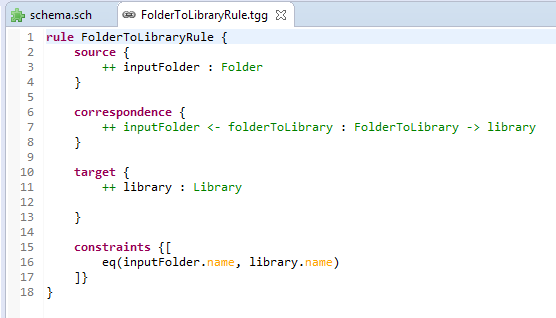
\includegraphics[width=\textwidth]{eclipse_FolderToLibraryRule}
  \caption{The TGG transformation will begin with this rule.}
  \label{eclipse:FolderToLibraryRule}
\end{center}
\end{figure}

\vspace{-0.5cm}

\subsubsection{ForAllShelfRule} % ---------------------------------

\item[$\blacktriangleright$] Let's use some elements from the previous rule to help us define how to handle creating shelves for our library. Copy and paste the
elements from each correspondence to a new \texttt{FolderToLibraryRule}, adding a \texttt{shelfFolder} and \texttt{shelf} and described in
Fig.~\ref{eclipse:ForAllShelvesRule}.

\vspace{0.5cm}

\begin{figure}[htbp]
\begin{center}
  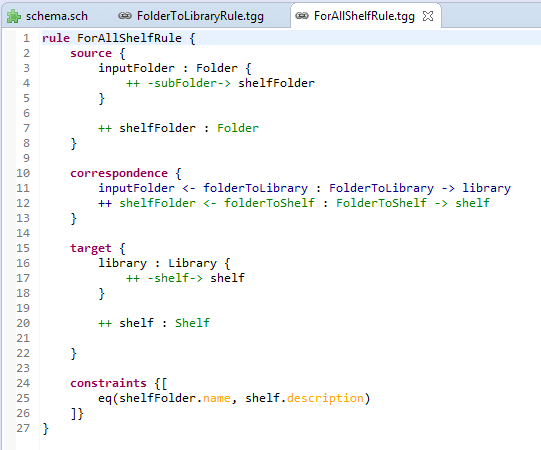
\includegraphics[width=0.9\textwidth]{eclipse_ForAllShelfRule}
  \caption{Completed \texttt{ForAllShelfRule}}
  \label{eclipse:ForAllShelvesRule}
\end{center}
\end{figure}

\item[$\blacktriangleright$] Don't forget that in order to successfully create the correspondence link between these elements, you need to add the
correspondence type to your \texttt{schema} (Fig.~\ref{eclipse:updatedSchema}).

\vspace{0.5cm}

\begin{figure}[h!]
\begin{center}
  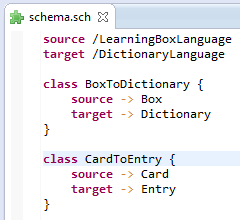
\includegraphics[width=0.7\textwidth]{eclipse_updatedSchema}
  \caption{Update the TGG \texttt{schema} with any new correspondence types}
  \label{eclipse:updatedSchema}
\end{center}
\end{figure}

\newpage

Now that we have the containers, we can handle the dictionary \texttt{File} elements. We know from our generated tree model that each dictionary will always
have a title node, but we're unsure if an author will be included, and we won't know how many entries are involved. Therefore, we should create at least three
different rules to handle this stage of the transformation. 

\subsubsection{NodeToDictionaryRule} % ---------------------------------

\item[$\blacktriangleright$] Create a rule name \texttt{NodeToDictionaryRule}, and build it as indicated in Fig.~\ref{eclipse:NodeToDictionaryRule}.

\vspace{0.5cm}

\begin{figure}[htbp]
\begin{center}
  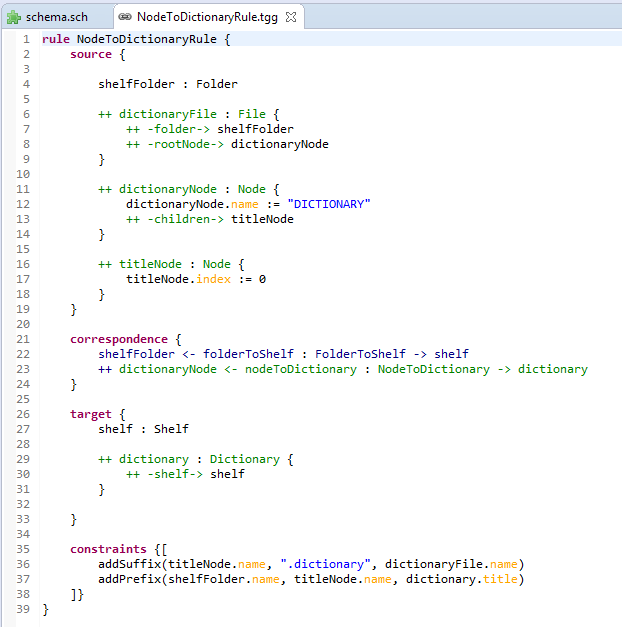
\includegraphics[width=\textwidth]{eclipse_NodeToDictionaryRule}
  \caption{\texttt{NodeToDictionaryRule} handling only \texttt{titleNode}s}
  \label{eclipse:NodeToDictionaryRule}
\end{center}
\end{figure}

\newpage

\item[$\blacktriangleright$] As you can see, this rule demands that a \texttt{shelfFolder} and \texttt{shelf} already exist before executing, implying that this
rule can only be called after executing \texttt{ForAllShelfRule}. An attribute constraint is used with \texttt{titleNode} to ensure that the correct child
\texttt{Node} is matched from \texttt{dictionaryNode}, and not accidentally to an author or entry node, which will have different indices.

\item[$\blacktriangleright$] This rule also imposes two constraints, one for each direction. In the forward transformation, we want to add the name of
the shelf to the dictionary file's title (i.e., ``english'' and ``numbers1-10'') and set it as the target's \texttt{name}. Though this may be somewhat abstract
at first, imagine this constraint is actually called ``add/remove Suffix'' since, during the inverse transformation, this constraint also will ensure the name
of the shelf is not present. Similarly, in the backwards transformation, the transformation needs to generate a valid \texttt{dictionaryFile} name, and it does
so by appending \texttt{.dictionary} to the end of \texttt{titleNode.name}.

\subsubsection{ForAllEntryRule} % ---------------------------------

\item[$\blacktriangleright$] Let's handle the \texttt{Entry} elements next. We can demand \texttt{Node\-To\-Dict\-ion\-ary\-Rule} be executed first by needing
context information from \texttt{dictionaryNode}. Create \texttt{ForAllEntryRule}, and build it so it matches
Fig.~\ref{eclipse:ForAllEntryRule}. Each \texttt{entryNode} will have a child \texttt{indexNode} and \texttt{contentNode} whose attribute constraints, and
transformation constraint ensure the correct information is set to its equivalent \texttt{entry} instance.

\begin{figure}[htbp]
\begin{center}
  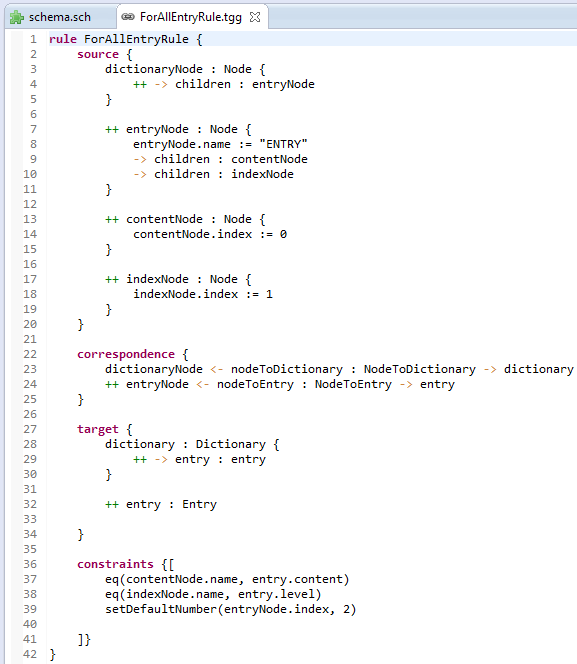
\includegraphics[width=\textwidth]{eclipse_ForAllEntryRule}
  \caption{Completed \texttt{ForAllEntryRule}}
  \label{eclipse:ForAllEntryRule}
\end{center}
\end{figure}

\newpage


The last thing we need to specify is how to handle \texttt{author}s. Transforming forwards from a \texttt{authorNode} to an \texttt{author} isn't as simple as
an \texttt{entryNode}, where you create an \texttt{entry} every time you find a valid match. Instead, we have to account for the possibility of a single author
for multiple dictionaries in a \texttt{Library}. While some users may not care about duplicate information, why not also provide a rule for the case when the
library needs to be optimized with only unique authors in a single \texttt{Library} instance?

\subsubsection{ForAllNewAuthorRule} % ---------------------------------

\item[$\blacktriangleright$] Create \texttt{ForAllNewAuthorRule}, and complete it as depicted in Fig.~\ref{eclipse:ForAllNewAuthorRule}. This is our one-to-one
correspondence rule, where every \texttt{authorNode} instance the rule is able to find, an equivalent \texttt{author} is created.

\begin{figure}[htbp]
\begin{center}
  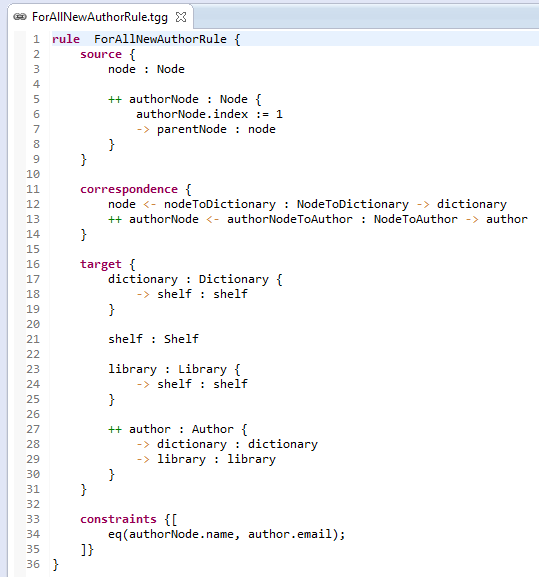
\includegraphics[width=\textwidth]{eclipse_ForAllNewAuthorRule}
  \caption{Creating new authors in \texttt{ForAllNewAuthorRule}}
  \label{eclipse:ForAllNewAuthorRule}
\end{center}
\end{figure}

\subsubsection{ExistingAuthorRule} % ---------------------------------

\item[$\blacktriangleright$] Similarly, create \texttt{ForExistingAuthorRule} as specified in Fig.~\ref{eclipse:ForExistingAuthorRule}. You should be able to
copy and paste the majority of the previous rule. In fact, the only thing you need to change are two small characters in front of \texttt{author} and its
\texttt{dictionary} reference, forcing the rule to assume and match to some context \texttt{author}, but still create a new link between the current dictionary
file and previous author.

\begin{figure}[htbp]
\begin{center}
  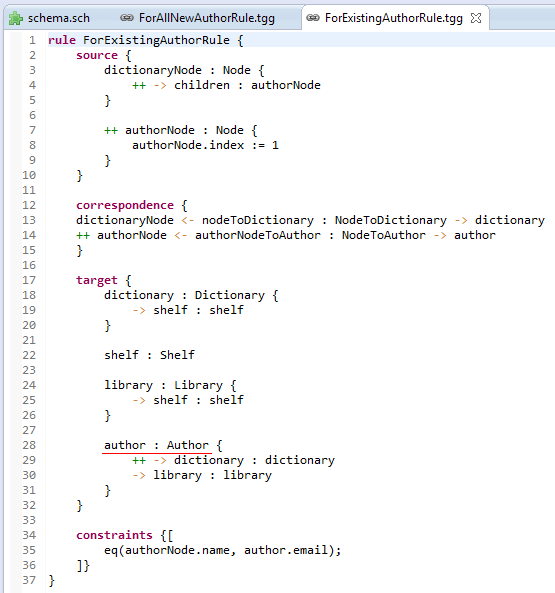
\includegraphics[width=\textwidth]{eclipse_ForExistingAuthorRule}
  \caption{Checking for existing authors in \texttt{ForExistingAuthorRule}}
  \label{eclipse:ForExistingAuthorRule}
\end{center}
\end{figure}

\newpage

\item[$\blacktriangleright$] Great work! You have now specified six different rules (with a focus on the forward direction) to perform a text-to-model
transformation! For confirmation, your final schema and package explorer should now resemble Fig.~\ref{eclipse:schemaFinal}.

\vspace{0.5cm}

\begin{figure}[htbp]
\begin{center}
  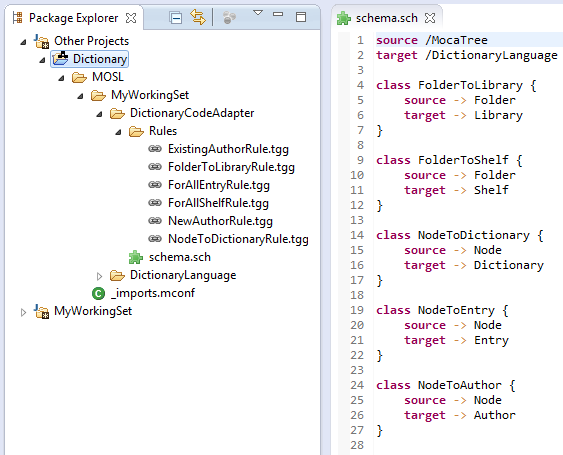
\includegraphics[width=\textwidth]{eclipse_finalSchema}
  \caption{Your final \texttt{rules} project structure and \texttt{schema}}
  \label{eclipse:schemaFinal}
\end{center}
\end{figure}

\vspace{0.5cm}

\item[$\blacktriangleright$] Given that everything has been done correctly, and MOSL hasn't reported any errors, build your TGG transformation. If
problems arise, be sure to double-check your files for spelling or character symbol mistakes.

\end{itemize}
